
\documentclass[UTF8]{ctexbeamer}

% There are many different themes available for Beamer. 
% A comprehensive list with examples is given here:
% http://deic.uab.es/~iblanes/beamer_gallery/index_by_theme.html
% You can uncomment the themes below if you would like to use a different

%\usetheme{AnnArbor}
%\usetheme{Antibes}
%\usetheme{Bergen}
%\usetheme{Berkeley}
%\usetheme{Berlin}
%%%%%
%\usetheme{Boadilla}
%%%%%
%\usetheme{boxes}
%\usetheme{CambridgeUS}
%\usetheme{Copenhagen}
%\usetheme{Darmstadt}
%%%%%
%\usetheme{default}
%\usetheme{Frankfurt}
%\usetheme{Goettingen}
%\usetheme{Hannover}
%\usetheme{Ilmenau}
%\usetheme{JuanLesPins}
%\usetheme{Luebeck}
%%%%%
%\usetheme{Madrid}
%\usetheme{Malmoe}
%\usetheme{Marburg}
%\usetheme{PaloAlto}
%\usetheme{Pittsburgh}
%\usetheme{Rochester}
%\usetheme{Singapore}
%\usetheme{Szeged}
%\usetheme{Warsaw}
\usetheme{Montpellier}

\title{YNU热点问题情感极性分析}

% A subtitle is optional and this may be deleted
\subtitle{——基于云南大学校园集市}

\author{AngLee} 

\institute[Universitiy]{
	2023 Spring MachineLearning Course\\
	YunNan University
 }
% - Keep it simple, no one is interested in your street address.

\date{开题报告 4.24}
% - Either use conference name or its abbreviation.
% - Not really informative to the audience, more for people (including yourself) who are reading the slides online

% If you have a file called "university-logo-filename.xxx", where xxx is a graphic format that can be processed by latex or pdflatex,then you can add a logo as follows:

\pgfdeclareimage[height=1.5cm]{university-logo}{ynu.jpg}
\logo{\pgfuseimage{university-logo}}

% Delete this, if you do not want the table of contents to pop up at the beginning of each subsection
\AtBeginSubsection[]
{
  \begin{frame}<beamer>{大纲}
    \tableofcontents[currentsection,currentsubsection]
  \end{frame}
}

% Let's get started
\begin{document}

\begin{frame}
  \titlepage
\end{frame}

\begin{frame}{大纲}
  \tableofcontents
\end{frame}


% Section and subsections will appear in the presentation overview and table of contents.
\section{选题背景}

\subsection{校园集市概述}
\begin{frame}{校园集市概述}
  \begin{itemize}
  \item {
    云南大学校园集市平台是云大师生进行求助和讨论的场所 }
  \item {
    通过对集市数据的分析,可以判断一段时间内学生的心理状况、监控对重大校园突发事件的舆论走向,即使发现心理问题,对于学生的心理健康和校园满意度有重大影响。
  }
  \end{itemize}
\end{frame}

\subsection{NLP情感极性分析}

\begin{frame}{NLP情感极性分析}
   \begin{itemize}
  \item {
    NLP即自然语言处理,Sentiment Analysis(情感极性分析)是自然语言处理的一个重要分支,通过分析文本信息,判断个人对事件的主观倾向:积极/消极,实现舆情监控和风险预警
  }
  \item {
    Sentiment Analysis经过多年的发展,发展出数据字典、机器学习、深度学习等多种分析方式
  }
  \end{itemize}
\end{frame}


% Section and subsections will appear in the presentation overview and table of contents.
\section{模型构建}

\subsection{数据来源}
\begin{frame}{数据来源}
  \begin{itemize}
  \item {
    数据获取:通过网络爬虫的方式,爬取云南大学校园集市的发帖信息,通过调用Paddle飞桨平台PaddleNLP API完成数据标注,构建训练集
  }
  \item {
    数据规模:受限于服务器限制,集市平台仅保留近一周的发帖数据,通过数据统计,近5天平均日发帖数量为150条,以30天作为数据获取周期,本项目的数据规模为4500条
  }
  \end{itemize}
\end{frame}

\subsection{模型选择}

\begin{frame}{模型选择}
   \begin{itemize}
  \item {
    实现Sentiment Analysis的方法众多,本次分别使用情感辞典,集成学习和深度学习的方式完成训练
  }
  \item {
    采用知网开源的情感辞典Hownet进行初步拟合
  }
  \item {
    采用集成学习的方式,使用adaboost将SVM和朴素贝叶斯两种弱分类器集成为强分类器,完成拟合
  }
  \item {
   采用LSTM深度学习模型进行拟合。由于不同词语对情感类别的影响不同,通过添加attention机制进行拟合
  }
  \end{itemize}
\end{frame}

\subsection{模型验证}
\begin{frame}{模型验证}
  \begin{itemize}
  \item {
    基于OpenAI gpt turbo 3.5 prompt的模型验证
  }
  \end{itemize}
\end{frame}




% Section and subsections will appear in the presentation overview and table of contents.
\section{项目创新}

\subsection{集成学习的使用}
\begin{frame}{集成学习的使用}
  \begin{itemize}
  \item {
    传统情感分析中,研究方向有传统机器学习领域和深度学习领域的两个方向,对于深度学习方向,新的成果层出不穷,而传统机器学习方向则更多的关注于如何优化单一的分类器以求得更好的效果,鲜有人使用继承学习的方式进行验证。
  }
    \end{itemize}
\end{frame}

\subsection{Attention机制的使用}
\begin{frame}{Attention机制的使用}
   \begin{itemize}
 \item {
    Attention机制是Transformer的核心思量,而后者则是GPT模型的基础,受限于硬件设备和数据集,我们无法复现GPT的训练过程,但通过在简单的情感分析任务中引入类似的Attention机制,完成分类任务,是对其内核的一次简单实践。
  }
  \end{itemize}
\end{frame}
  
\subsection{调整prompt验证模型}

\begin{frame}{调整prompt验证模型}
   \begin{itemize}
 \item {
    通过调用OpenAI gpt turbo3.5,拟合不同prompt对验证结果的影响
  }
  \end{itemize}
\end{frame}



% Section and subsections will appear in the presentation overview and table of contents.
\section{进度和难点}

\subsection{进度}
\begin{frame}{进度}
  \begin{itemize}
  \item {
    通过Charles抓包,初步分析了校园集市平台的http包交互逻辑,通过无头浏览区构建了相应的header,抓取了简单的数据
  }
  \item {
    对于SVM,朴素贝叶斯等构建了相应的实现方式
  }
   \end{itemize}
\end{frame}

\subsection{难点}

\begin{frame}{难点}
   \begin{itemize}
  \item {
    集市平台采用Vue架构,html骨架和层叠样式表以及javascript的结构不熟悉,需要花费一定的时间解析
  }
  \item {
    对于LSTM和attention机制的应用难度较大,需系统性的研读相关论文
  }
  \end{itemize}
\end{frame}



% All of the following is optional and typically not needed. 
\appendix
\section<presentation>*{\appendixname}
\subsection<presentation>*{项目结构}

\begin{frame}[allowframebreaks]
  \frametitle<presentation>{|项目结构}
 \begin{figure}[htbp]
  \centering
  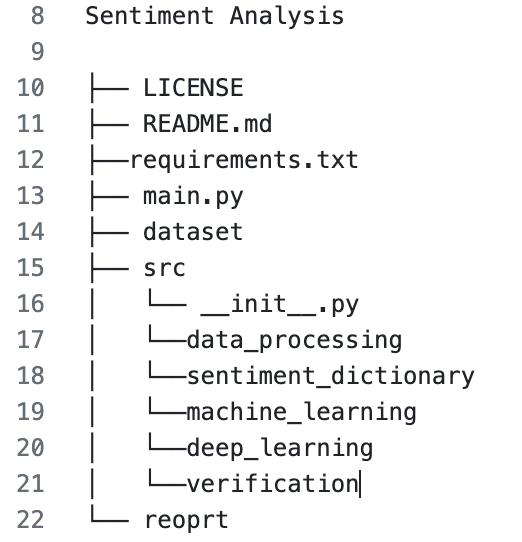
\includegraphics[width=0.5\textwidth]{structure.png}
  \caption{文件组织结构}
  \label{fig:example}
\end{figure}
\end{frame}

\subsection<presentation>*{开源地址}

\begin{frame}[allowframebreaks]
  \frametitle<presentation>{|开源地址}
  https://github.com/anglee2002/SentimentAnalysis
\end{frame}

\end{document}


